\documentclass[a4paper,12pt]{article}

\usepackage{latexsym}
\usepackage[utf8]{inputenc}
\usepackage[T1]{fontenc}
\usepackage{graphicx}
\usepackage{amsmath}
\usepackage{float}
\usepackage{textcomp} % for Number (\textnumero) symbol
\usepackage[hidelinks]{hyperref}

\author{Krzysztof~Palka and Dominik~Odrowski}
\date{April 29, 2013}

\title{\textsc{Exercise} 351 \\
Electron motion in electric and magnetic fields} 

\addtolength{\textwidth}{2.5cm}
\addtolength{\hoffset}{-1.25cm}

\begin{document}

    \maketitle

    \begin{abstract}
        This report presents measurement of the electron's charge/mass ratio.
    \end{abstract}

    \section{Introduction}
    The aim of this exercise was to determine, using longitudinal magnetic field method, the electron's charge/mass ratio and to get acquaint with action of magnetic field on charged particles. 

    \section{Theory and measurement}

    Because of Lorenz's force charged particles are affected by magnetic field. Charged parallel plates also can affect movement of charged particles -- because of electric field. Those properties are used in this experiment. Electrons released by cathode are accelerated and formed into beam by anode. Then they are deflected by parallel plates by electric field. Because of present magnetic field (form coil) which is parallel to direction of movement of accelerated particles, if they are deflected then start spiral motion (helical trajectory). When reaching the screen, electrons could be in different distance form X axis, but they are in the same phase of rotary motion and we can observe a line on screen. In some situations if angle of deflection is 0 or $\pi$ Lorenz force doesn't occurs and we see one point on screen.
    We can describe this situation with equation 
    \begin{equation}
        x = v_x nT = v_x n \frac{2 \pi m}{e B}
    \end{equation}
    We can measure particular currents for coil for particular accelerating voltage, and basing on that using following formula calculate ratio of charge $e$ of electron to it's mass $m$.    

    \begin{equation}
        \frac{e}{m} = \frac{8 \cdot \pi^2 \cdot n^2 \cdot U}{x^2 \cdot B^2} \label{eq:general}
    \end{equation}
    
    \begin{figure}[H]
    \begin{center}
        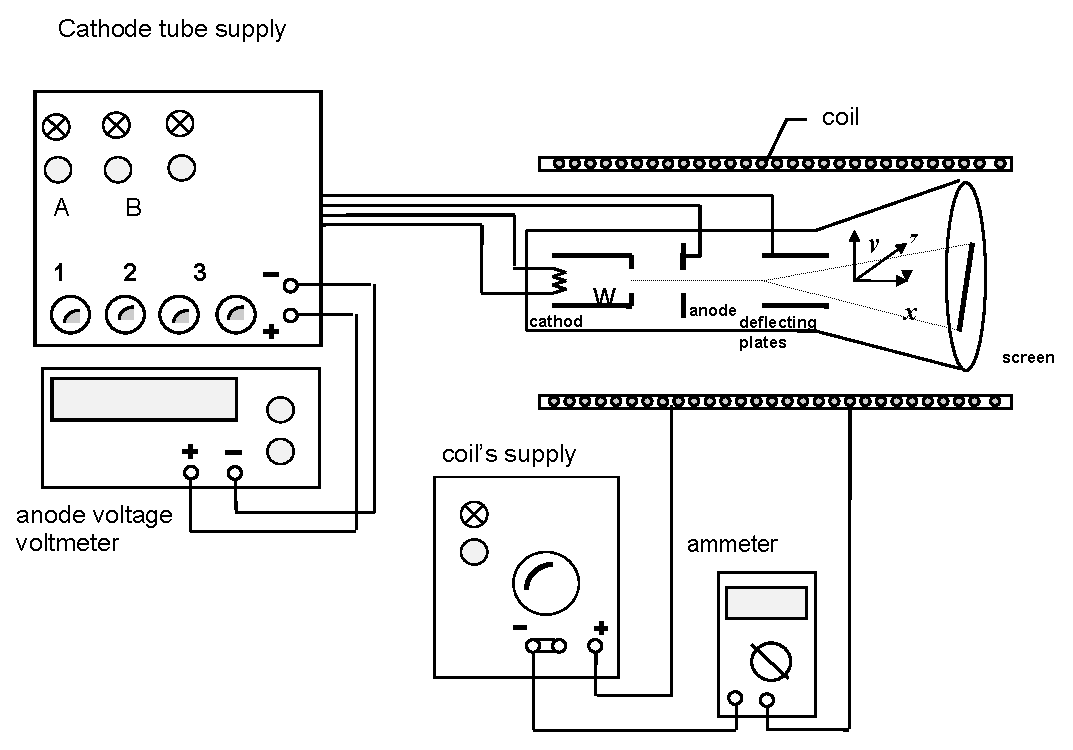
\includegraphics[width=0.75\textwidth]{set-up}
        \caption{Experimental setup}
        \label{fig:set-up}
    \end{center}
    \end{figure}


    \section{Results}

    Values of magnetic induction -- $B$ and $B^2$ can be calculated form following equation \cite{E17}:
    \begin{equation}
        B = \frac{\mu_0 \cdot \mu \cdot I \cdot N}{2\cdot \sqrt{\left(r + \frac{h}{2} \right)^2 + \frac{L^2}{4}}}
    \end{equation}
    where $\mu_0 = 4 \pi \cdot 10 ^{-7}$ [V\,s\,A$^{-1}$\,m$^{-1}$] - magnetic permeability of vacuum; $\mu$ = 1 - relative magnetic permeability of the air; $I$ - current int the coil circuit; $N$ = 2215; $r$ = 0.04[m] - coil's radious; $h$ = 0.009[m] - thickness of coil turns and $L$ = 0.3[m] - length of the coil.
    

    As measurements of $I_2$ and  $I_3$ were less accurate (there was a wider range of current in which we couldn't distinguish whether we still see a point or a line) we have calculated value of $B$ only for $I_1$.

    \begin{table}[H]
        \begin{center}
            \caption{Measured coil current -- $I_1$, $I_2$ and $I_3$ for set accelerating anode voltage $U$ and calculated magnetic induction values $B$ and $B^2$}
            \label{tab:results}
            \begin{tabular}{|c|c|c|c|c|c|c|}
                \hline
                \textnumero 
                & $U$ [V]
                & $I_1$ [A] & $I_2 [A] $ & $I_3 [A]$
                & $B$ [$10^{-3}$ T]
                & $B^2$ [$10^{-7}$ T] \\
                \hline
                1 & 341 & 0.63 & 1.25 & 1.83 & 5.60 & 3.14\\
                2 & 390 & 0.68 & 1.33 & 1.96 & 6.05 & 3.65\\
                3 & 440 & 0.71 & 1.42 & 2.11 & 6.31 & 3.98\\
                4 & 490 & 0.73 & 1.51 & 2.25 & 6.49 & 4.21\\
                5 & 540 & 0.79 & 1.58 & 2.30 & 7.02 & 4.93\\
                6 & 590 & 0.84 & 1.63 & 2.53 & 7.47 & 5.58\\
                7 & 640 & 0.86 & 1.73 & 2.53 & 7.65 & 5.85\\
                8 & 690 & 0.89 & 1.79 & 2.68 & 7.91 & 6.26\\
                9 & 740 & 0.93 & 1.83 & 2.76 & 8.27 & 6.84\\
                10 & 790 & 0.97 & 1.91 & 2.83 & 8.62 & 7.44\\
                11 & 821 & 0.97 & 1.92 & 2.90 & 8.62 & 7.44\\
                \hline
            \end{tabular}
        \end{center}
    \end{table}

    We have placed this data, more specifically, accelerating anode voltage and magnitude of magnetic induction squared and plot of linear regression by least squares method on following graph.   

    \begin{figure}[H]
    \begin{center}
        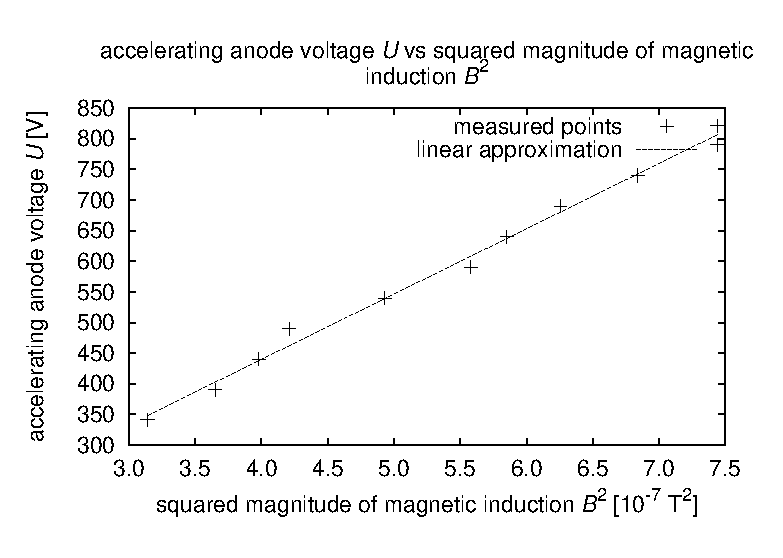
\includegraphics[width=0.75\textwidth]{graph}
        \caption{Graph of $U(B^2)$ and linear approximation for measured points.}
        \label{fig:graph}
    \end{center}
    \end{figure}

    We have obtained slope (assuming that $U = aB^2)$ $a = (1.07 \pm 0.03) \cdot 10^{7} \frac{\mathrm{V}}{\mathrm{T}^2}$

    By dependency from equation \ref{eq:general} we can obtain:
    \begin{equation}
        U = \frac{x^2}{8\pi^2 n^2}\frac{e}{m}{B^2} \label{eq:U}
    \end{equation}
    where $n$ is order of focusing, 1, and length of the electron's path inside the cathode tube is $x = 0.072$ [m].  

    Because factors $U$ and $B^2$ occurs in both \ref{eq:general} and \ref{eq:U} equations we can find that 
    \begin{equation}
        \frac{m}{e} = a \cdot \frac{8\pi^2 n^2}{x^2}
    \end{equation}
    so propagation of error in this case would be 
    \begin{equation}
        \Delta \frac{e}{m} = \left(\frac{\Delta x}{x} + \frac{\Delta a}{a}\right) \cdot \frac{e}{m}
    \end{equation}
    where $\Delta x = 0.004$[m].
    So the final result is 
    \begin{displaymath}
        \frac{e}{m} = (1.6\pm0.2) \cdot 10^{11} \frac{\mathrm{C}}{\mathrm{kg}}
    \end{displaymath}
    

    \section{Conclusions}
    According to \cite{HRW} $e/m_e = 1.76 \times 10^{11}$ C/kg. This result is within boundaries of our error, but this error is quite big. We think that the main reason of this was impossibility to find accurate value of current which led to quite big Asymptotic Standard Error for linear regression (about 3\%). And of course one of the factors was error of experimental set-up ($\Delta x$) itself.  

    \begin{thebibliography}{9}
        \bibitem{E17}\emph{Exercise 17. Electron motion in electric and magnetic fields} (2005) [online]. Bogdan Żółtowski. Pracownia Fizyki Współczesnej Instytutu Fizyki PŁ. Łódź. Available online at: \url{http://phys.p.lodz.pl/materialy/mdems/351.pdf}. Accessed May 8, 2013.
        \bibitem{HRW}\emph{Fundamentals of physics} (2011) [ebook]. David Halliday, Robert Resnick, Jearl Walker. 9th ed. ISBN 978-0-470-46908-8

    \end{thebibliography}

\end{document}

